\section{Impermeable Particle near a Permeable Layer: Spectra, Crossovers and Transparency}\label{sec:rigid}

Isolating the hydrodynamic signature of the porous substrate by considering an impermeable no-slip sphere ($\kappa=1$,
$\hat\ell_c=0$) reveals how finite permeability reshapes both dissipation and added mass across the transition from
viscous to inertial flow.

\subsection{Interaction spectra from the viscous to the inertial regime}\label{sec:spectra}

\begin{figure*}[t]
  \centering
  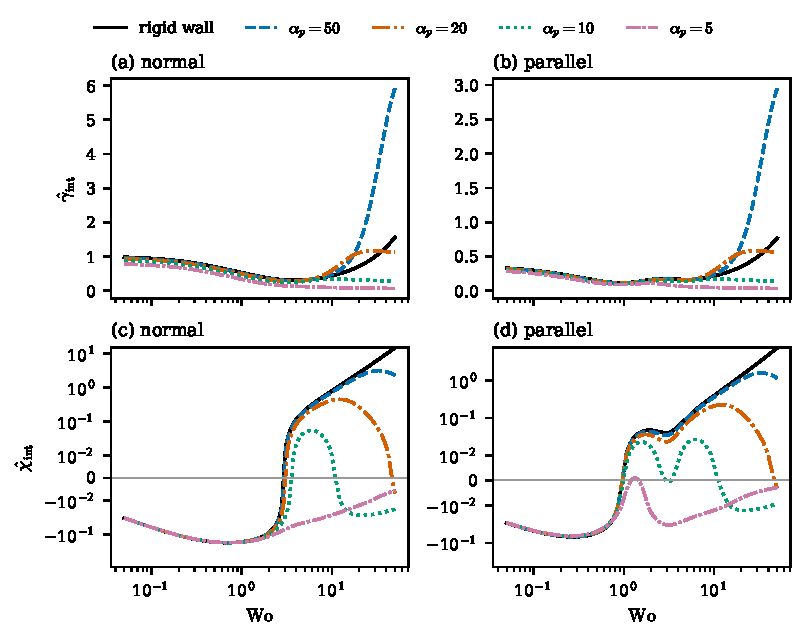
\includegraphics[width=\linewidth]{figures/fig3_spectra.pdf}
  \caption{Interaction spectra of an impermeable sphere at $\varepsilon=1$ and $\beta_p=0$, for a rigid wall and for
  layers with $\alpha_p=50,20,10,5$. (a,b) Wall-induced damping $\hat\gamma_{\rm int}$ against $\Wo$. (c,d) Reactive
  coefficient $\hat\chi_{\rm int}=\omega m_{\rm int}/(6\pi\mu b)$ against $\Wo$, on a symmetric logarithmic axis that is
  linear for $|\hat\chi_{\rm int}|<10^{-2}$; its sign is that of $m_{\rm int}$. (a,c) Normal, (b,d) parallel oscillation.
  Note the single sign change near a rigid wall, the second (downward) sign change for permeable layers, and the
  double positive window in (d) for $\alpha_p=10$.}
  \label{fig:spectra}
\end{figure*}

Near a rigid wall, the wall-induced added mass is negative at low frequency and positive at high frequency, as shown by
the solid black curves in \cref{fig:spectra}(c,d). At $\varepsilon=1$, the reactive coefficient $\hat\chi_{\rm int}$
changes sign once, at $\Wo_c=2.92$ in normal oscillation and at $\Wo_c=0.955$ in parallel oscillation. Above the crossover,
$m_{\rm int}$ approaches the positive inviscid image value of \cref{eq:inviscid}; below it, the negative sign is opposite
to that of any inviscid image, pointing to a viscous origin. In an unbounded fluid, the term $-6\pi\lambda$ in $Z_U$
represents the frequency-domain form of the Basset history force~\cite{maxey1983equation}, whose reactive component
$6\pi\Wo/\sqrt2$ is carried by vorticity diffusing over the distance $|\lambda_f|^{-1}$ during one oscillation period.
When $|\lambda_f|^{-1}$ exceeds the gap, this vorticity reaches the wall and is annihilated there. The computed spectra
confirm this mechanism quantitatively: as $\Wo\to0$, $-\hat\chi_{\rm int}$ approaches the full unbounded Basset term
$\Wo/\sqrt2$, with the ratio $-\hat\chi_{\rm int}/(\Wo/\sqrt2)$ reaching $0.99$ (normal) and $0.96$ (parallel) at
$\Wo=0.01$ and $\varepsilon=1$, before decreasing as $\delta_v$ shrinks below the gap. \finding{The negative added mass at
low $\Wo$ is therefore the part of the Basset memory force that the wall removes. It is the frequency-domain counterpart
of the wall-induced change in the long-time velocity tail of a Brownian sphere analysed by
Felderhof~\cite{felderhof2005effect}, which has been observed with optical tweezers by Mo et
al.~\cite{mo2015broadband}.} Under the resonance-shift relation of \cref{sec:nondim}, this sign change reproduces
qualitatively the crossover of the AFM frequency shift reported by Zhang et al.~\cite{zhang2023unsteady}; for a colloidal
probe of radius $b=10\,\mu$m in water, $\Wo_c=2.92$ corresponds to a linear frequency $f=\omega/(2\pi)\approx14$\,kHz,
well within the operating range of colloidal-probe AFM. The rigid-wall damping $\hat\gamma_{\rm int}$ in
\cref{fig:spectra}(a,b) follows a distinct trend, falling from its steady value $0.98$ to a minimum of $0.31$ near
$\Wo\approx3.7$ before rising again as the Stokes boundary layer of thickness $\delta_v$ on the wall thins and dissipates
more energy.

\begin{figure}[t]
  \centering
  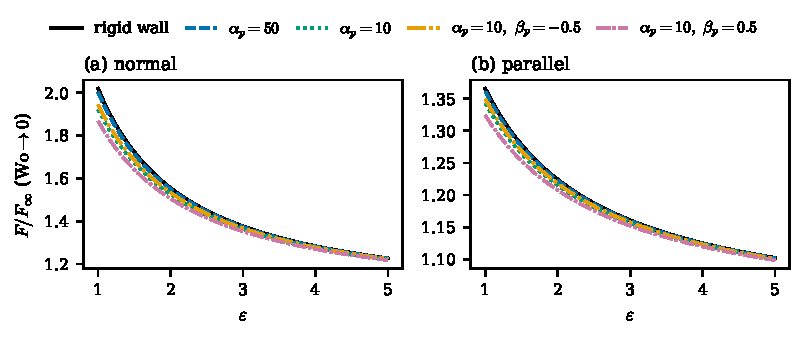
\includegraphics[width=\linewidth]{figures/fig4_steady.pdf}
  \caption{Steady ($\Wo\to0$) resistance $F/F_\infty$ of an impermeable sphere against the gap $\varepsilon$, for a
  rigid wall and for layers with $\alpha_p=50$ and $10$ and stress jumps $\beta_p=\pm0.5$. (a) Normal, (b) parallel
  oscillation.}
  \label{fig:steady}
\end{figure}

Introducing finite substrate permeability weakens the steady interaction only modestly while fundamentally altering the
high-frequency response. In the steady limit ($\Wo\to0$), fluid escapes into the porous half-space, reducing
$\hat\gamma_{\rm int}(\Wo\to0)$ in normal oscillation from $0.98$ for the rigid wall to $0.94$, $0.89$, and $0.78$ for
$\alpha_p=20$, $10$, and $5$, respectively. As shown in \cref{fig:steady}---which recovers the normal-motion problem of
Faltas et al.~\cite{faltas2021axisymmetric} and extends it to parallel motion---the total steady resistance
$F/F_\infty$ at $\varepsilon=1$ drops by only a few per cent, from $2.018$ (rigid wall) to $1.921$ for $\alpha_p=10$ in
normal motion and from $1.365$ to $1.342$ in parallel motion. Varying the stress jump at $\alpha_p=10$ shifts the normal
resistance to $1.867$ for $\beta_p=0.5$ and to $1.943$ for $\beta_p=-0.5$, and all curves merge for
$\varepsilon\gtrsim4$, demonstrating that steady drag is a weak probe of substrate permeability. At finite frequency,
however, \cref{fig:spectra}(a,b) shows that the damping departs from the rigid-wall curve and passes through a pronounced
maximum at $\Wo=O(\alpha_p)$. On an extended frequency range, this peak occurs at $\Wo=9.8$, $29.6$, and $105$ for
$\alpha_p=10$, $20$, and $50$, corresponding to $\Wo/\alpha_p=1.0$--$2.1$. For $\alpha_p\ge20$, the peak exceeds the
rigid-wall damping at the same frequency, by a factor of $2.2$ for $\alpha_p=50$ ($\hat\gamma_{\rm int}=6.7$ against
$3.1$). \finding{The maximum appears where the viscous penetration depth becomes comparable with the Brinkman screening
length $\sqrt{k_p\mu_p/\mu}$ of the layer, so that the oscillatory flow enters the layer and does work against its Darcy
drag. This dissipation channel is absent at a rigid wall, and it also governs the unsteady flow next to an oscillating
porous wall studied by Sherwood~\cite{sherwood2020unsteady}.} We note this mechanism as a physical interpretation
consistent with the peak location rather than a derived asymptotic result. Simultaneously, in \cref{fig:spectra}(c,d),
the reactive coefficient for $\alpha_p=5$ remains negative across all frequencies, eliminating the positive-added-mass
window altogether.

\subsection{Crossover map and the transparency law}\label{sec:woc}

\begin{figure*}[t]
  \centering
  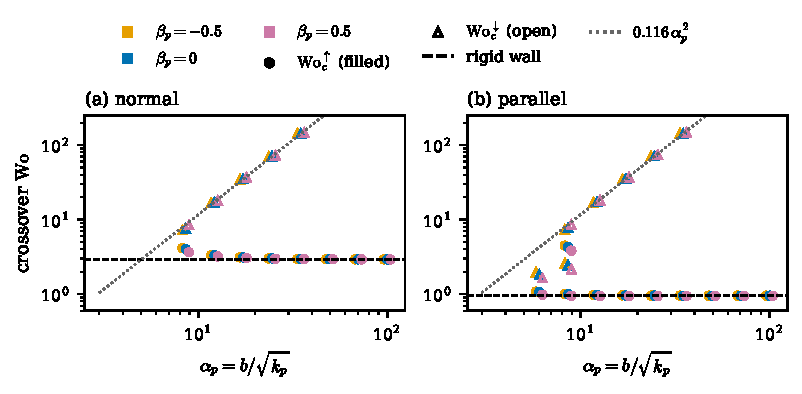
\includegraphics[width=\linewidth]{figures/fig5_crossovers.pdf}
  \caption{All crossover Womersley numbers of $m_{\rm int}$ against the layer permeability $\alpha_p$ at
  $\varepsilon=1$, for $\beta_p=-0.5,0,0.5$ (markers offset slightly in $\alpha_p$ for visibility). Filled circles:
  upward crossovers $\Wo_c^{\uparrow}$; open triangles: downward crossovers $\Wo_c^{\downarrow}$. Dashed: rigid wall.
  Dotted: $\Wo_c^{\downarrow}=0.116\,\alpha_p^2$. Downward crossovers above the scanned range
  $\Wo\le\max(150,2.5\alpha_p)$ are not shown. (a) Normal, (b) parallel oscillation.}
  \label{fig:woc_ap}
\end{figure*}

Collecting every sign change of $m_{\rm int}$ in \cref{fig:woc_ap} shows that substrate permeability both raises the lower
upward crossover $\Wo_c^{\uparrow}$ and introduces a gap-independent upper downward crossover $\Wo_c^{\downarrow}$. In
normal oscillation with $\beta_p=0$, $\Wo_c^{\uparrow}$ increases from $2.92$ for the rigid wall to $2.96$, $3.10$, $3.31$,
and $4.01$ for $\alpha_p=35$, $17$, $12$, and $8.6$, with the shift steepening as the layer becomes more permeable so that
$\Wo_c^{\uparrow}$ is most sensitive for $\alpha_p\lesssim30$. A positive stress jump, which facilitates tangential
momentum transfer into the layer, lowers $\Wo_c^{\uparrow}$ (from $4.14$ for $\beta_p=-0.5$ to $3.64$ for $\beta_p=0.5$ at
$\alpha_p=8.6$), though its influence fades for $\alpha_p\gtrsim30$. Above the positive-added-mass window, every finite
$\alpha_p$ introduces a downward crossover $\Wo_c^{\downarrow}$ beyond which $m_{\rm int}$ becomes negative again.
Numerically, $\Wo_c^{\downarrow}/\alpha_p^2$ remains within $0.112$--$0.116$ for $\alpha_p\ge12$ (a least-squares fit
gives $\Wo_c^{\downarrow}\propto\alpha_p^{2.08}$), and varying the gap alters $\Wo_c^{\downarrow}$ by less than $3\%$: at
$\alpha_p=17.3$, $\Wo_c^{\downarrow}=34.7$, $35.3$, and $35.5$ for $\varepsilon=1$, $2$, and $3$, and at $\alpha_p=24.6$ it
equals $70.2$, $71.2$, and $71.5$. \finding{For $\mu_p=\mu$ and $\beta_p=0$, this quadratic transparency law follows
directly from a high-frequency asymptotic expansion for $\Wo\gg\alpha_p\gg1$. In this regime, reflected vorticity at
$\bx_0$ is exponentially small and the interaction is governed by the potential image $F_{\rm int}\approx Z_pU_p$. For
wavenumbers $k=O(h^{-1})\ll\Wo$, continuity of normal stress and normal velocity across $z=0$ yields the potential
reflection coefficient
$R_\Phi\approx(c_3-c_1)/(c_3+c_1)=i\alpha_p^2/(2\Wo^2)+\alpha_p^4/(4\Wo^4)+O(\alpha_p^6/\Wo^6)$, while
\cref{eq:rigid_BC,eq:rigid_Z} give $Z_pB=-i\pi\Wo^2[1+3\sqrt2(1+i)/\Wo+O(\Wo^{-2})]$. Because $U_p\propto-R_\Phi B/h^3$,
the leading $O(\alpha_p^2/\Wo^2)$ imaginary part of $R_\Phi$ produces Darcy damping, whereas the reactive force
$\hat\chi_{\rm int}$ is set by the competition between the $O(\alpha_p^4/\Wo^4)$ real part of $R_\Phi$ (positive added
mass) and the product of the $O(\Wo^{-1})$ viscous boundary-layer phase of $Z_pB$ with the $O(\alpha_p^2/\Wo^2)$
imaginary part of $R_\Phi$ (negative added mass). Balancing these two terms,
$\alpha_p^4/(4\Wo^4)=3\sqrt2\,\alpha_p^2/(2\Wo^3)$, yields the closed-form transparency law
\begin{equation}
  \Wo_c^{\downarrow}=\frac{\alpha_p^2}{6\sqrt2}\approx0.1179\,\alpha_p^2,
  \label{eq:transparency}
\end{equation}
which matches the numerical prefactor $0.116$ to within $2\%$ and, because the geometric factor $h^{-3}$ and directional
image prefactor cancel identically, explains why $\Wo_c^{\downarrow}$ is independent of the gap $\varepsilon$ and
identical for normal and parallel oscillation.} In dimensional form, \cref{eq:transparency} corresponds to
$\omega\approx\mu b^2/(72\rho k_p^2)$, extending to a finite particle the high-frequency transparency of an unsteady
Brinkman wall~\cite{sherwood2020unsteady}.

As $\alpha_p$ decreases further, the upward and downward crossovers approach each other and coalesce, closing the
positive-added-mass window completely between grid points for $6.1<\alpha_p<8.6$ in normal oscillation and
$4.3<\alpha_p<6.1$ in parallel oscillation; below this threshold, $m_{\rm int}$ remains negative at every frequency,
while a positive $\beta_p$ widens the window (raising $\Wo_c^{\downarrow}$ from $7.19$ to $8.40$ at $\alpha_p=8.6$). In
parallel oscillation near the threshold ($\alpha_p=8.6$ and $10$), \cref{fig:spectra}(d) and \cref{fig:woc_ap}(b) reveal
that the positive window splits into two separate intervals, exhibiting four sign changes of $m_{\rm int}$ (at
$\Wo\approx0.97$, $2.88$, $3.26$, and $11.3$ for $\alpha_p=10$), a feature that persists unchanged on a 120-point grid
with doubled quadrature. Decomposing the reactive force of \cref{eq:response} into its potential-image part $Z_pU_p$ and
its vortical-reflection part $Z_ww_0$ clarifies the origin of this split. \finding{In parallel motion, the reflected
vorticity produces a positive reactive force near $\Wo\approx1$ that decays once the viscous penetration depth becomes
smaller than the gap, whereas the potential image is negative at low $\Wo$ and turns positive only at higher frequency.
Near a rigid wall, the image turns positive ($\Wo\approx2.6$) before the vortical contribution has decayed, yielding a
single window; a permeable layer weakens the image and delays its sign change ($\Wo\approx3.4$ for $\alpha_p=10$), so that
the sum returns to zero between the two contributions. The split thus reflects the separation of the viscous-memory and
inviscid added-mass parts of the unsteady force~\cite{mazur1974generalization,maxey1983equation}.} In normal oscillation,
the vortical contribution is weaker relative to the potential image and no split occurs. Taken together, the two
crossovers offer a non-contact, gap-independent measure of substrate permeability: a frequency sweep at fixed
$\varepsilon$ yields $\Wo_c^{\uparrow}$ (sensitive for $\alpha_p\lesssim30$) and $\Wo_c^{\downarrow}$ from
\cref{eq:transparency}, which requires no knowledge of the gap. For a probe of radius $b=10\,\mu$m in water near a
hydrated airway mucus layer (whose typical mesh pore sizes of 100--500\,nm correspond to $\sqrt{k_p}\sim0.1$--$0.5\,\mu$m),
$\alpha_p=20$ ($\sqrt{k_p}=0.5\,\mu$m) gives $\Wo_c^{\downarrow}\approx46$ ($f\approx3.4$\,MHz), well within the range of
ultrasonic and acoustofluidic excitation; for the much denser endothelial glycocalyx (where $\sqrt{k_p}$ is typically
2--3\,nm), achieving comparable $\alpha_p$ requires nanometric probes and correspondingly higher frequencies.
